\documentclass{article}
\usepackage[utf8]{inputenc}
\usepackage[left=3cm,top=3cm,right=3cm,bottom=3cm]{geometry}
\newcommand*\chem[1]{\ensuremath{\mathrm{#1}}}
\usepackage{amsmath}
\usepackage{mathtools}

\usepackage{natbib}
\usepackage{graphicx}

\let\oldthebibliography\thebibliography
\let\endoldthebibliography\endthebibliography
\renewenvironment{thebibliography}[1]{
  \begin{oldthebibliography}{#1}
    \setlength{\itemsep}{0em}
    \setlength{\parskip}{0em}
}
{
  \end{oldthebibliography}
}

\begin{document}

\begin{center}
\Huge
Identificación y exfoliación de monocristales de calcogenuros de metales de transición unidimensionales.

\vspace{3mm}
\Large Jesús David Rincón Puche

\large
201126021

\Large José Alejandro Montaña Cortés
\large 


\vspace{2mm}
\Large
Director: Paula Giraldo Gallo\\


\normalsize
\vspace{2mm}

\today
\end{center}

\begin{abstract}
 En este proyecto se caracterizará las propiedades químicas de metales de calcogenuros de transición unidimensionales para poder estudiar 
\end{abstract}

\normalsize
\section{Introduction}

Superconductivity (SC) is one of the most spectacular quantum effects in condensed-matter physics. This phenomenon consists of a material presenting no resistivity and expelling all the magnetic fields that act upon it, allowing the electric current to flow without dissipation~\cite{Leggett}. Thanks to this, it has a great potential for applications such as levitating trains~\cite{Trains}, magnetic resonance imaging~\cite{Resonance}, among many others. There are several characteristics involving 
materials that feature this effect: First their transition temperature, $T_c$, to the superconducting phase is a fraction of the Fermi degeneracy temperature, $T_f$, and the Cooper pairs, two electrons that form a bound state due to an effective attraction, are distributed among the lattice. Also, it is believed that the mechanism underlying this indirect coupling is the exchange of virtual phonons. Furthermore, several of them can be understood under the Bardeen, Cooper and Schrieffer (BCS) theory~\cite{PhysRev.108.1175}.

Even though this phenomenon has been studied rigorously, a complete understanding is lacking. For example, in strongly correlated systems, SC competes with other quantum effects generated by correlations such as the Charge Density Wave (CDW), which occurs when the charge density has a periodic behavior in the lattice, prominently in low dimensional systems~\cite{CDW}, which weakens the SC phase. It has been observed in both  experiments~\cite{Competition1} and theoretical studies based on mean-field theory~\cite{MeanField} that doping can strengthen the SC phase, by weakening the CDW. Motivated by these observations, the main purpose of this project is to study theoretically the competition between SC and CDW in highly interacting systems, when varying the filling to simulate  doping, going beyond mean-field by considering correlations.  This study will be perfomed using the extended Fermi Hubbard Hamiltonian, a very simple model that contains the competition of interest and has been studied extensively, using the Density Matrix Renormalization Group (DMRG) algorithm. The following section will present studies done on some materials that inspire this project as well as theoretical studies that serve as foundation. Afterwards, the Hamiltonian and algorithm to be used will be explained.

\section{State of the art}
\subsection{Experimental and theoretical studies}

Some of the materials that have received a lot of attention recently, and where the SC and CDW competition has been studied extensively are the transition metal chalcogenides. These are constituted by one transition metal and a number of calchogens (two calchogens make a dichalcogenide, for example), and are interesting materials for the study of optical physics in the field of photonics and optoelectronics applications as well as nanoelectronics~\cite{dical}. Additional to this, these materials are extremely sensitive to external perturbations which leads to large changes in their physical properties~\cite{dical}. This make them very attractive systems to understand the competition that occurs among these phases~\cite{dical}, and since they do not have magnetic states, and possess a low critical temperature~\cite{MeanField}, the study of this competition becomes simpler when compared to cuprates, that are high temperature superconductors but present phases with magnetic order. Furthermore, some experimental studies have shown that when the dichalcogenide is doped, the CDW or the SC get stronger, depending on the type of doping~\cite{Competition1}. The latter consists of maintaining the same number charge of carriers by changing the original chalcogen and doping with a different metal, or replacing the metal for one of identical valence. 

These properties are present in most of the families of these materials, particulary in the trichalcogenides, which corresponds to quasi 1D layered materials that have an unique chain-like structure~\cite{trical} and are very useful for applications in field-effect transistors, infrared, visible and ultraviolet photodetectors, and for the next generations in electronics~\cite{trical}. Since they are 1D materials, they can present unique properties such as the so-called Luttinger Liquid or Spin Charge Separation~\cite{Giamarchi}, resulting in very rich and interesting effects.

Although there are many models used to study SC, the Fermi Hubbard is one particular choice of many studies because in spite of its simplicity, it contains a lot of rich physics, including the SC-CDW competition. Previous studies on very small Fermi Hubbard lattices~\cite{quarterfilling} have suggested that the superconducting phase takes place over a broader area when the system is at quarter filling when compared to half filling (same number of spin up and spin down particles in the lattice, with zero magnetization). This result was obtained from the charge gaps in each region, since in the CDW there is an energy cost at introducing an extra charge to the system, in contrast to SC. Recently~\cite{MeanField}, a simulation based on mean field was made on a model of dichalcogenides using the Extended Fermi Hubbard model. It was observed that the addition of disorder weakens the CDW phase generating islands where the SC phase is stronger. This study, however, is limited for its use of mean field theory, which does not take spatial correlations in consideration. 

Based on these studies, an analysis on how varying from half filling to quarter filling slowly using DMRG, is necessary. This method captures spatial correlations and simulate large system correctly, giving far more information on the competition between SC and CDW and how to optimize SC.

\subsection{Extended Fermi-Hubbard Hamiltonian}

The Extended Fermi-Hubbard Hamiltonian is a simple model that contains the competition between SC and CDW, which is frequently used to help unravel the complex physics of strongly correlated systems. This is given by:

\begin{equation}
    H=-J\sum^{N-1}_{i,\sigma}{(c^{\dagger}_{i,\sigma}c_{i+1,\sigma} + H.c)}+U\sum^{N}_{i=1}{n_{i,\downarrow}n_{i,\uparrow}} + V\sum^{N-1}_{i,\sigma,\sigma'}{n_{i,\sigma}n_{i+1,\sigma'}},
\end{equation}

where $\sigma$ represents the direction of the spin, either down ($\downarrow$) or up ($\uparrow$); $N$, the number of sites in the lattice, $c_{i,{\sigma}}$ and $c^{\dagger}_{i,{\sigma}}$ represent the annihilation and creation operators, respectively, for a fermion at site $i$ with spin $\sigma$; h.c, the hermitian conjugate of this operator, and $n_{i,\sigma}$, the local density operator defined as $n_{i,\sigma}=c^{\dagger}_{i,{\sigma}}c_{i,{\sigma}}$. In addition, $J$ is the hopping interaction between nearest neighbors; $U$, the local Coulomb interaction and $V$, the nearest neighbor Coulomb interaction. Figure \ref{phaseDiag} shows the ground state phase diagram of this Hamiltonian at half filling.

\begin{figure}
    \centering
    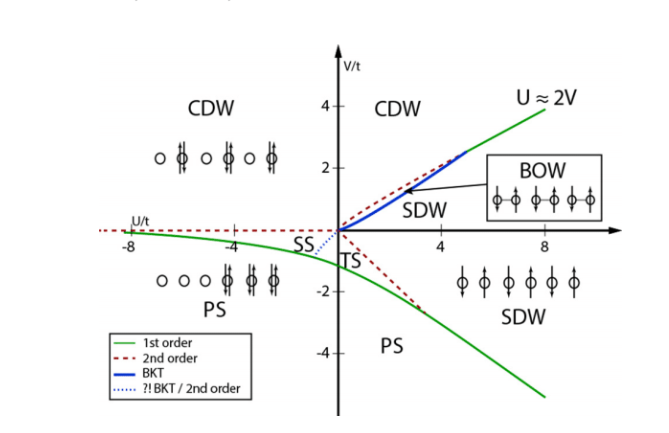
\includegraphics[scale=0.7]{phaseDiagramaHalfFilling.PNG}
    \caption{Phase Diagram of the Extended Fermi Hubbard Model. Taken from \cite{Diagram}}
    \label{phaseDiag}
\end{figure}

Given the effects of interest of the current project, our focus is on the weak coupling limit, attractive $U$ and different values of $V$. In particular,  the CDW phase is divided in two zones: Repulsive interaction between neighbors with local attraction and, both repulsive with $V>>U$. In the first zone, the local Coulomb attraction prompts the electrons to form double occupancies in one site, while the nearest neighbor interaction repels them from going to another site. In the second zone, the stronger neighboring repulsion naturally induces the charge periodicity~\cite{Diagram}.

In the singlet SC phase (SS) both interactions are attractive, $U<0$ and $V<0$, prompting the electrons to form pairs. This means these fermions are interacting in an indirect way. That interaction is contained in $V$, which is the so-called effective potential proposed in the BCS model~\cite{PhysRev.108.1175,Clase} that allow indirect interactions between electrons forming Cooper pairs. On the other hand, in the weak coupling limit when $U>0$ and $V<0$, a Triplet SC (TS) region is formed. ~\cite{Diagram}. 

The model feautures other interesting phases, which even though are not the object of the present proposal, are worth mentioning. One is "Phase Separation" (PS), here both $V$ and $U$ are highly attractive making all the electrons cluster as close as possible~\cite{Diagram}. Another one is, the Spin Density Wave (SDW) which takes place in $U>0$ so the local repulsion takes prominence, leading to the antiferromagnetic ordering shown~\cite{Diagram}. Lastly is the Bond Order Wave (BOW) which possess alternating  strengths  of  the  expectation  value  of  the  kinetic energy  operator on  the  bonds, for intermediate values of $U$ and $V$~\cite{Diagram}.
 
\subsection{DMRG algorithm}

The Density Matrix Renormalization Group (DMRG) is the most powerful numerical method to study strongly correlated 1D systems. The purpose of the algorithm is to find the ground state of the system of study by minimizing the energy~\cite{DMRG}. The main qualities of this method are the ability to simulate large systems, something that cannot be done using exact diagonalization, that it does not have the fermionic sign problem, which occurs in quantum Monte Carlo~\cite{DMRG}, and captures correctly spatial correlations going beyond the capabilities of mean field theory~\cite{DMRG}.

In highly correlated systems, certain properties are achieved that allow the success of this method. First, most of the elements of the Hamiltonian matrix are zero, allowing the system to be truncated, since most of the information is contained in few eigenvalues of the density matrix.

Secondly, a bipartition of the system, $A$ and $B$, is proposed. With this bipartition, the entropy of entanglement, namely the von Neumann entropy, which measures quantum correlations between subsystems, is used to as proxy quantity to determine said eigenvalues. This is defined as~\cite{DMRG}

\begin{equation}
    S=-\sum_iw_iln(w_i),
\end{equation}

where $w_i$ are the eigenvalue of the reduced density matrix of one of the subsystems. In the boundary of the subsystems, the so-called area laws predict that for ground states of short ranged Hamiltonian, this entropy if proportional to the surface, $dL$, where $L$ corresponds to the dimension of the system, in which the system is contained, rather than $L$; in 1D systems, $S$ is constant because the surface in 1D system is equivalent to a point~\cite{DMRG,ORUS2014117}, signifying that the correlations across the system do not grow arbitrarily, but are bounded, and thus can be characterized efficiently.

\subsubsection{MPS and MPO}

We describe the basic ideas of DMRG using the language of Matrix Product States (MPS). For this, some linear algebra concepts need to be introduced. 

Singular Value Decomposition (SVD), for any matrix C of size $m\times n$ is defined as:

\begin{equation}
    C=USV^{\dagger},
\end{equation}

where $U$ is a matrix of $m\times p$ size;$p$, the $\min{m,n}$; S, a diagonal $p\times p$ matrix size and $V^\dagger$ is of size $p\times n$. The elements associated to $S$ are known as the singular values of the matrix, which will be denoted as $S_a$. Also, $U$ and $V^\dagger$ have the normalization properties:

\begin{equation}
    I=U^{\dagger}U, \quad I=V^{\dagger}V,
\end{equation}

where $I$ is the identity matrix. Consider a state $|\psi>$, and the bipartition, $A$ and $B$. In this situation, the state can be written as

\begin{equation}
    |\psi>=\sum^{d^l}_{i=1}\sum^{d^{N-l}}_{j=1}\Psi_{ij}|i>_A|j>_B
\end{equation}

where the coefficients $\Psi_{i,j}$ indicate the elements of a matrix, and are the amplitude of probability in each combination of states. When applying a SVD to this matrix, the result is

\begin{equation}
    \Psi_{i,j}=\sum^{\chi}_{a=1}U_{i,a}S_aV^T_{a,j},
\end{equation}

where $\chi$ is the size of the $S$ matrix. Replacing in the state gives

\begin{equation}
    |\psi>=\sum^{\chi}_{a=1}S_a|A>_a|B>_a.
\end{equation}

Here $S_a$ is always ordered from highest to lowest values. Additionally, the new states are defined as:

\begin{equation}
    |A>_a=(\sum^{d^{l}}_{i=1}U_{i,a}|i>_A) \quad |B>_a=(\sum^{d^{N-l}}_{j=1}V^T_{a,j}|j>_B)
\end{equation}

The normalization of the state implies that:

\begin{equation}
    1=\sum^{\chi}_{a=1}S_a^2.
\end{equation}

From equation (7) is natural to imagine that the state can be approximated by truncating the number of singular values in the expansion, namely as $|\psi>\ \simeq |\psi'>$, where $|\psi'>$ is defined as,

\begin{equation}
    |\psi'>=\sum^{\chi'}_{a=1} S_a|A>_a|B>_a
\end{equation}

with $\chi'<\chi$. Thus the error associated to the truncation is:

\begin{equation}
  \epsilon=\sum^{\chi}_{i=\chi'+1}S_a^2,
\end{equation}

It turns out that this can be done with a very low error in 1D systems with short-range Hamiltonians, because of the bounded behavior of correlations resulting from the area law, as mentioned before.

Now, these truncation ideas can be applied to a general many-body system state of the form

\begin{equation}
    |\psi>=\sum^{d}_{n_1,...,n_L=1}C_{n_1,...,n_L}|n_1,...,n_L>,
\end{equation}

where $C_{n_i}$ is the amplitude of probability in each state and $|n_i>$ is the basis for each site in the lattice. When reshaping $C_{n_1},...,{n_L}$, then applying SVD to it and repeating the process, it can be shown that~\cite{ORUS2014117}  

\begin{equation}
    |\psi>=\sum_{n_1,...,n_L} A^{n_1}...A^{n_L}|n_1,...,n_L>,
\end{equation}

where the coefficient is rewritten as a product of matrices. This structure is known as a Matrix Product State (MPS).

This description has a nice graphical representation, whose building blocks are depicted in figure \ref{Tensor}

\begin{figure}
    \centering
    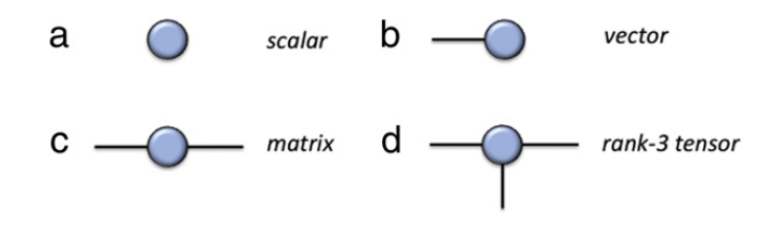
\includegraphics[scale=0.7]{TensorMPS.PNG}
    \caption{Building blocks of a MPS\cite{ORUS2014117}}.
    \label{Tensor}
\end{figure}

Here, we can see how each tensor is defined as one circle with a defined number of legs. For example a matrix, which is a grade 2 tensor, has two legs. With this representation, several matrix operations can be depicted. Since a tensor contraction is represented by connected legs, Figure\ref{Blocks}, shows several tensorial products.

\begin{figure}
    \centering
    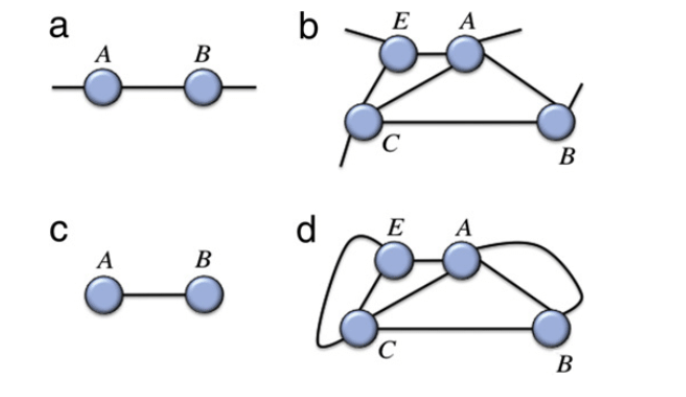
\includegraphics[scale=0.6]{TensorProduct.PNG}
    \caption{Graphical representation of tensorial product using. Taken from \cite{ORUS2014117}}.
    \label{Blocks}
\end{figure}

We can see in figure~\ref{Blocks}.a, the product of two matrices. In this case, each element connects one leg, leaving two legs free, thus reaming a matrix in the end. In \ref{Blocks}.c, on the other hand, the representation is a dot product, since the elements connect their only leg to create a scalar. This process can be done with the other two images, which are higher grade tensors (\ref{Blocks}.d, is an scalar because it has no free legs).

\begin{figure}
    \centering
    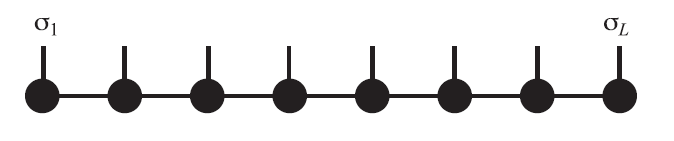
\includegraphics[scale=0.5]{MPS.PNG}
    \caption{Graphical representation of a MPS-Taken from \cite{DMRG}}.
    \label{MPS}
\end{figure}

Figure~\ref{MPS} shows the graphical representation of a MPS. The tensor of each site, $A^{n_i}$ is constituted by three legs. The lateral legs correspond to the interacting between other tensor and the vertical leg is the reduce Hilbert space for that state.

The idea of DMRG within the MPS language is to determine the matrices, $A^{n_i}$, that for a given Hamiltonian, H, minimize the energy, $E=<\psi|H|\psi>$, which is performed as a variational process~\cite{DMRG,ORUS2014117}.

\subsection{Mechanisms of study}

The purpose is, as mentioned before, to use DMRG to obtain ground states of different values of $U$ and $V$ and various fillings, and see how SC and CDW compete in each case. To determine the phase of each set of parameters, different quantities will be calculated. First, the charge gap is defined as~\cite{quarterfilling}

\begin{equation}
    \Delta_{charge}=E(L;N+1)+E(L;N-1)-2E(L;N)
\end{equation}

where $E$ is the energy in the ground state for a certain filling; L, the total number of sites in the lattice and N the total number of particles in the system. As mentioned in section 1.2, this is a key parameter to determine the superconducting phase in a quantitative way. This gap represents the energy to add or remove one electron in the ground state, compared to the system with no alterations. The reason this quantity can show the separation between phases, is that in the SC there is no energy cost at introducing an extra charge to the system in contrast to CDW. 

Additional to this, another form to characterize each phase corresponds to spatial correlations. In particular, we are interested in the correlations for superconductivity, which are defined as

\begin{equation}
    S_{singlet}=\frac{1}{\sqrt{N}}\sum_{i}c_{i,\uparrow}c_{i+x,\downarrow}-c_{i,\downarrow}c_{i+x,\uparrow}
\end{equation}

where $x$ is the separation between sites. In addition, for CDW, the order parameter is defined as~\cite{Diagram}

\begin{equation}
    O_{cdw}=\frac{1}{N}\sum_{m,n}e^{ik(m-n)}[<n_mn_n>-<n_m><n_n>],
\end{equation}

where $n_m=n_{m,\downarrow}+n_{m,\uparrow}$ and $m$ and $n$ represent sites in the system. Both correlations demand a lot of computational resources. However, quantum entanglement is a good tool to determine criticallity in a system,  since it has been able obtain phase diagrams of several models such as the extended Fermi Hubbard with the exception of the subtle transition between Singlet and triplet SC phase, as well as the SDW and BOW transition~\cite{Diagram}. The measure of quantum correlations will be calculated as indicated in equation (2).

\section{Objectives}
\subsection{General Objective}

To study how changing the filling in the extended Fermi Hubbard Hamiltonian affects SC and CDW, using the DMRG algorithm. 

\subsection{Specific Objectives}

\begin{enumerate}
    \item To develop a DMRG code and to test it by comparing the simulations to known results
    \item  To calculate, using charge gaps and quantum entanglement, critical points between SC and CDW while varying filling.
    \item To determine the parameter regimen values that optimizes SC.
\end{enumerate}

\section{Methodology}

As mentioned in sections 1 and 2, this work will be perfomed using DMRG. First initialization files created from MatLab and then uploaded to the university cluster to simulate the ground state for different values of $U$ and $V$ in the left zone of the diagram~\ref{phaseDiag}. From these simulations, charge gap, correlation functions and entanglement will be calculated. This information will be analyzed to determine the parameter regimen values that optimizes SC.

\section{Ethical considerations}

All the data that will be used in this project will be properly cited acknowledging the work done by other authors. Since this is a theoretical work, it does not need to go the Ethical Committe of the Science Faculty of the University.

\section{Chronogram}

\begin{table}[htb]
	\begin{tabular}{|c|cccccccccccccccc| }
	\hline
	Task $\backslash$ weeks & 1 & 2 & 3 & 4 & 5 & 6 & 7 & 8 & 9 & 10 & 11 & 12 & 13 & 14 & 15 & 16  \\
	\hline
	1 & X & X & X & X &   &   &   &  &  &   &   &   &   &   &   &   \\
	2 &   & X & X & X  & X & X &  &   &   &  &  &  &   &  &  &   \\
	3 &   &   &   &   &   & X  & X  & X & X  & X  & X  & X &  X &   &  &   \\
	4 &  &  &  &  &  &  &  & X & X & X &  X & X  &  X & X  &  X &   \\
	5 &   &   &   &   &  &   &   &   &  & &  X & X &  X & X & X &   \\
	6 &   &   &   &   &  &   &   &   &  &   &   & X &  X & X  & X & X  \\
	\hline
	\end{tabular}
\end{table}
\vspace{1mm}

\begin{itemize}
	\item Task 1: Literature survey on DMRG and Extended Fermi Hubbard Hamiltonian.
	\item Task 2: Development and testing of DMRG code 
	\item Task 3: Simulation of ground states for different fillings and values of $U$ and $V$
	\item Task 4: Calculation of gaps, correlations and entanglement based on the results of the simulations.
	\item Task 5: Determination of phase diagram for each filling.
	\item Task 6: Write final document and publishable article.
\end{itemize}

\section{Experts in the field}

\begin{itemize}
    \item Luis Quiroga Puello (Universidad de Los Andes)
    \item Edgar Patiño (Universidad de Los Andes)
    \item Jereson Silva (Universidad Nacional de Colombia)
\end{itemize}

\section*{Firma del Director}
\vspace{1.5cm}

\section*{Firma del Codirector}
\vspace{1.5cm}

\bibliographystyle{unsrt}
\bibliography{references}
\end{document}



